%%%%%%%%%%%%%%%%%%%%%%%%%%%%
%%%%%%%%%%%%%%%%%%%%%%%%%%%%
\section{Detection of conflicting signal} \label{sec:extensions}

Consensus trees assumes congruence among trees in the set. Trees that turn out to be far away from the consensus tree can be the sign of high variance or conflicting signals. While high variance implies weak phylogenetic signal, conflicting  signals implies incongruence. Most distance distances, such as RF, are discrete and lead to very coarse distance distributions. By contrast, continuous distances are a simple way to characterize variance and distinguish one from the other. Moreover continuous distance lend themselves nicely to standard aspects of inferential statistics such as confidence sets and hypothesis testing. 

%Consider the space tree
%\begin{itemize}
% \item BHV space topology
% \item Means and variances in the tree space \textcolor{red}{briefly mentioned in previous section}
% \item Multivariate Analysis based on tree distances
% \end{itemize}

The  geometric  model of \cite{Billera2001} allows one to compare phylogenetic  trees,  with  the  same  leaf  set  of  cardinality $m$, in a quantitative way.  This  space  has  a  natural  metric, giving a way of measuring distance between phylogenetic trees and providing some procedures for averaging or combining several trees whose leaves are identical. This geometry also shows which trees appear within a fixed distance of a given tree and enables construction of convex hulls of a
set of trees. It also provides a justification for disregarding portions of a collection of trees that agree,  thus simplifying the space in which comparisons are to be made.

%%%%%%%%%%%%%%%%%%%%%%%%%%%%
\subsection{Tree Space definition} \label{sec:Tree-distances}
 The distance $d(T_i,T_j)$ between two trees $T_i$ and $T_j$ account for differences with respect to both their tree topologies (branching structure) and branch lengths. The space is constructed by representing each of the $(2m-3)!!$ possible tree topologies by a single non-negative Euclidean orthant of dimension $m-3$ (the largest possible number of internal branches). The orthants are then “glued together” along appropriate axes. Specifically, nearest neighbor interchange (NNI) topologies lie in adjacent non-negative orthants along the boundary corresponding to the collapse of the relevant NNI edge.

For two trees with different topologies, the BHV distance is the length of the shortest path between them that remains in the treespace.  The length of any path can be computed by calculating the Euclidean distance of the path restricted to each orthant that it passes though, and summing these lengths.  The shortest path is called a geodesic, and will pass from one orthant to the next orthant through lower-dimensional boundaries corresponding to trees with fewer splits. Since the space is nonpositively  curved, the geodesics are unique. 

\begin{figure}
 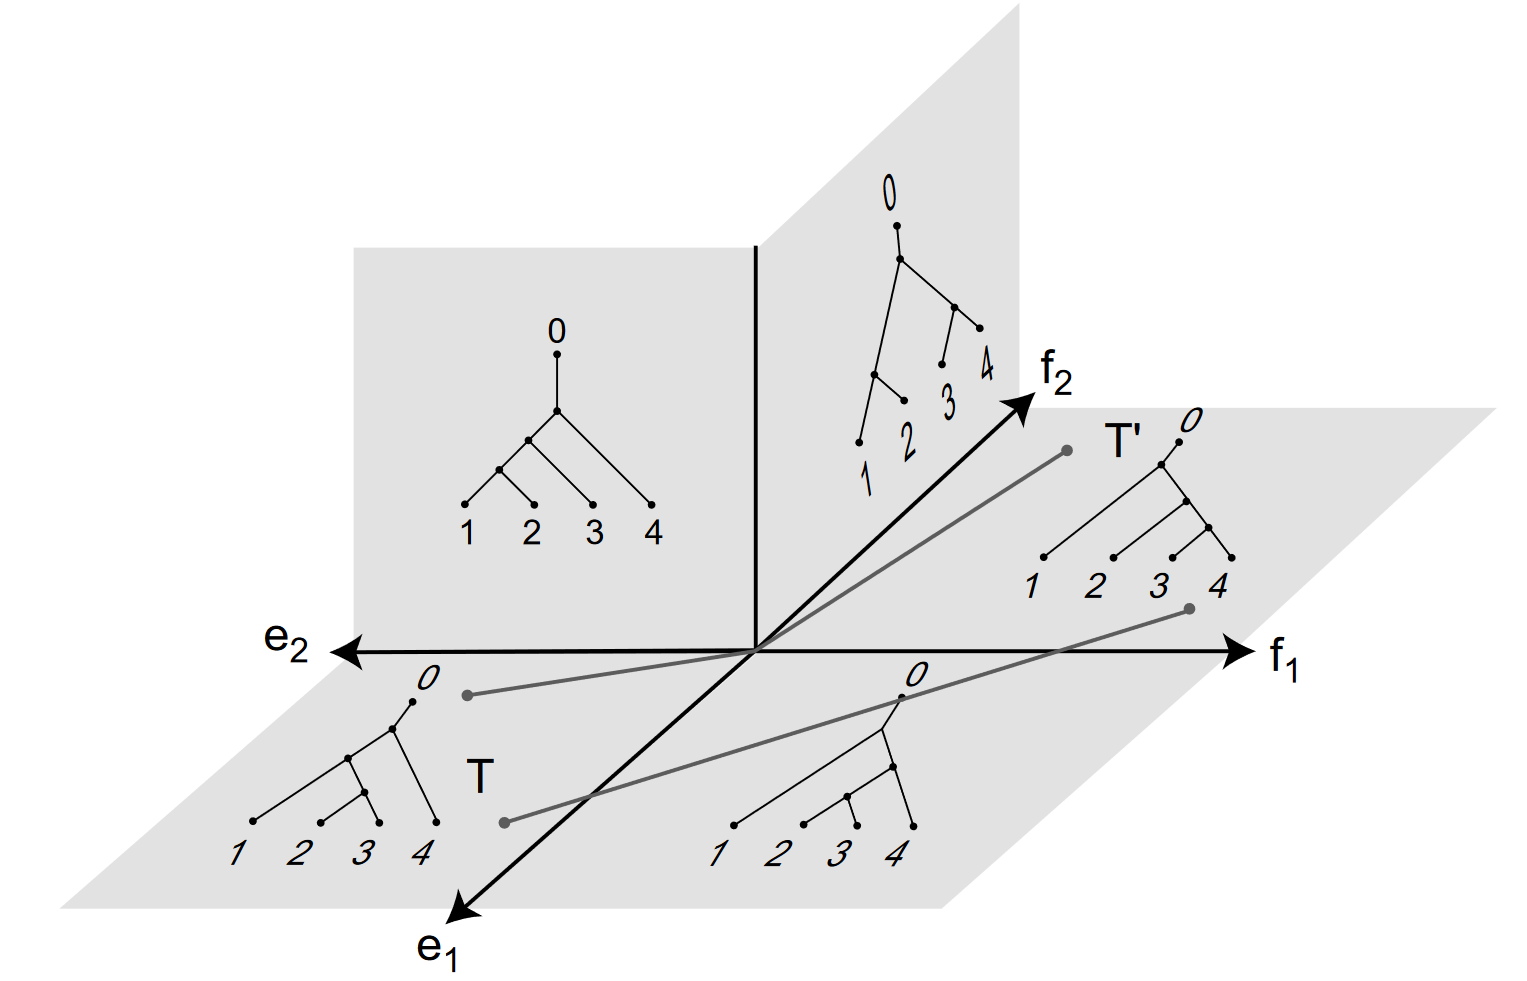
\includegraphics{Figs/OrthantBHV}
 \caption{Orthants in the BHV space (one per topology) and geodesic paths between two trees corresponding to topologies $T$ and $T'$. Reproduced from \citet{Billera2001}.}
\end{figure}

In Euclidean space, the Fr\'echet mean is the point minimizing the sum of the squared distances to the sample points, and is equivalent to the coordinate-wise average of the sample points. The mean tree is not necessarily a refinement of the majority-rule consensus tree. Fr\'echet variance is the tree that minimize the sum of squared distances.  This variance is unique because treespace is non-positively curved. The Fr\'echet variance of a set of trees quantifies how spread out a set of trees is from their mean. See \cite{miller2015polyhedral,brown2017mean} for details.

%%%%%%%%%%%%%%%%%%%%%%%%%%%%
\subsection{Use of BHV distance} \label{sec:means-and-variance}

\cite{barden2017logarithm} proved a Central Limit Theorem on the BHV treespace, showing that the distribution of the sample means converges to a certain Gaussian distribution. It is useful for detecting splits of weak and strong support and in tree-valued hypothesis testing.

A key tool of \cite{barden2014limiting}is  the log map  that permits to  map  trees  from  their  metric  space  to  Euclidean space, where it is possible to model a tree estimate $\hat T$ as a noisy realization of the true tree $T$. Once  the model parameters are estimated, Euclidean multivariate analysis techniques to reduce the dimension of the trees can be used. This allows to visualize tree estimates, along with their uncertainties.

For example it is possible to use the variance covariance matrix to  estimate  the  principal  directions  of  variability  via principal components analysis. The axes of the $\mathbb{R}^m$ ellipsoid indicate the relative directions of precision, and the ellipsoid can be shrunk  to be wholly contained in the same orthant as $\hat T_n$. This gives an unambiguous indication of the relative
confidence in the edges of the estimated tree. Note that the procedure is unambiguous about the trees contained in the confidence set for a given confidence level $\alpha$ (see \cite{willis2016confidence}).

Recently, \cite{de2012phylo} developed a statistical non-parametric method to detect outlier trees from the set of gene trees. They first convert gene trees into vectors in a multidimensional Euclidean space and then apply multiple co-inertia analysis (MCOA)—an extension of principal coordinate analysis—directly to these vectorized gene trees. Their method, Phylo-MCOA, also detects outlier species, those whose position varies widely from tree to tree. Included in our results are simulation studies comparing our non-parametric method with Phylo-MCOA.

\cite{weyenberg2014kdetrees}  proposes  a non-parametric estimator of the distribution that generated the sample trees $T_1,\ldots,T_n$.  This estimator can be viewed as a refined version of histogram-based estimation of a density. The kernel function, is a non-negative function defined on pairs of trees, which measures how similar two trees are. Kernel density estimation use the fact that points close to sample points tend to have higher likelihood than distant outlier points.  The ultimate goal is to detect outlier trees, $T_j$, which are not actually drawn from the true distribution.
%%%%%%%%%%%%%%%%%%%%%%%%%%%%
%\subsection{Confidence Sets Based on other Distances} \label{sec:kernel}
%
%Kernel based methods (using a distance matrix) to find outlier and build confidence sets.

%%%%%%%%%%%%%%%%%%%%%%%%%%%%
\subsection{Need for a Strong Theoretical Framework} 

With the democratization of high-throughput sequencing, acquiring new genome data has ceased to be the limiting factor in phylogenetic, except maybe for organisms that are difficult to sample from the environment. In contrast, phylogeneticists are now faced with a rise in data errors, which stems from a flood of increasingly bogus genomic data that has become intractable by hand. Given the size of current and upcoming phylogenomic datasets (thousands of genes for hundreds —   and soon thousands —   of species), computational requirements are emerging as the new limiting factor. As multiple possible improvements are theoretically able to limit systematic error (and artefacts) during phylogenetic inference, we  need  to determine the set of properties that the ideal model of sequence of evolution should combine.  An alternative approach is to use robustness methods to downweight or discard portions of the data where model misspecification occurs potentially mitigating the estimation biases these data may incur. This latter, in combination with improved models, may ultimately allow the development of robust and efficient analytical
tools that are also computationally tractable. 